\documentclass[man]{apa2}
\usepackage{pslatex}
\usepackage{amssymb}
\usepackage{graphicx}
\usepackage{color}
\usepackage{covington}
\usepackage[usenames,dvipsnames]{xcolor}

\title{Young children's developing sensitivity to discourse continuity as a cue for inferring reference}

\twoauthors{Alexandra C. Horowitz}{Michael C. Frank}
\twoaffiliations{Department of Psychology, Stanford University}{Department of Psychology, Stanford University}


\abstract{Children learn some words in simple situations where both a novel word and a cue to its meaning coincide in time. In many conversations, however, these sources of information are not presented simultaneously, but may instead occur in succession within a discourse.  We therefore investigated children's ability to use discourse information to connect a novel word with its referent. In Experiment 1, we created an ambiguous word-learning situation in which two novel toys were described. A novel label was embedded between two utterances that both referred to one of the two toys. Children three years old and older were more likely to attribute the label to the toy whose descriptions surrounded the naming event. In Experiment 2, to test the extent to which this inference relied on simpler heuristics such as temporal association, a new group of participants heard a label that was introduced after two utterances about the same toy (rather than between the two utterances). Both children and adults responded close to chance with this modification. Together these results suggest that discourse continuity is a reliable cue to reference that can be used to guide listeners' inferences in word learning.

~\\

Keywords: discourse; word-learning; language development; pragmatics}

\shorttitle{Discourse as a Cue for Inferring Reference}
\rightheader{Discourse as a Cue for Inferring Reference}

\acknowledgements{Special thanks to the staff and families at the San Jose Children's Discovery Museum. This work supported by a John Merck Scholars Fellowship to MCF. An earlier version of this work was presented to the Cognitive Science Society in \citeA{horowitz2013}.

~\\

\noindent Address all correspondence to Alexandra C. Horowitz, Stanford University, Department of Psychology, Jordan Hall, 450 Serra Mall (Bldg. 420), Stanford, CA, 94305. Phone: 650-721-9270. E-mail: \texttt{ahorowit@stanford.edu}}

\begin{document}

\maketitle                            


\section{Introduction}

Children can use many strategies to learn new words.  In overtly pedagogical situations, adults employ cues like pointing and other signals of joint attention to establish reference, helping children to learn word meanings \cite{bakeman1984,csibra2010,hollich2000}.  Many situations do not feature unambiguous ostensive cues at all times, however. If children are to learn in these more ambiguous cases, they must rely on other strategies to infer the meanings of novel words. Here we consider discourse structure---the order of utterances and how they relate to each other---as a cue. We focus particularly on \emph{discourse continuity}, the idea that sentences in close succession are more likely to relate to the same topic. The current study measures children's ability to use discourse continuity to make inferences about the referent of novel words in simple, grounded contexts.

Children are exposed to information about discourse structure whenever they hear speech, and the simple linking of topics across sentences could provide a valuable source of information about the meanings of words. From an utterance such as

\begin{example}
I love chinchillas!
\end{example}

\noindent a child may not be able to infer what ``chinchilla'' means. But consider this same utterance as embedded in a short discourse:

\begin{example}
\label{ex:chin}
I got a new pet. \\ I love chinchillas! \\ They're so soft.
\end{example}

\noindent When a locally ambiguous utterance is supported by a discourse structure that provides information about the topic (whatever is referred to by the word ``chinchilla''), the child can infer (A) that a chinchilla is a pet, and (B) probably a furry one.  The linking of information across a sequence of utterances requires that children have some understanding of discourse structure.  For inference (A), the child must assume that the statement in the second utterance is topically related to the first, and for inference (B), the child must assume that the pronoun in the third co-refers to the noun in the second. 

We focus here on inferences like (A). We begin by discussing adults' recognition of discourse structure cues and how these abilities may relate to children's language processing; we then discuss links between these abilities and word learning. Our review of previous literature sets the stage for our experiment, which tests whether adults and children are able to make a simplified version of this inference, using an assumption of discourse continuity to infer which object a novel term refers to.
 
Throughout this discussion, the perspective we take on word learning is that there are (at least) two problems that learners jointly solve during word learning \cite{frank2009,mcmurray2012}. First, the problem of in-the-moment referential ambiguity, and second, the longer-term problem of finding the conceptual extension of a word (even when its referent is known). We refer to the first problem as the problem of determining reference, and the second problem as the generalization problem. Although (2) highlights the potential of discourse information for both problems, we begin by considering the role of discourse in referent selection.\footnote{A somewhat orthogonal concern about calling this word learning has to do with children's retention of the referents they select. Some recent work indicates that although young children can use in-the-moment information to make inferences about reference, mappings inferred in this way are not necessarily retained \cite{horst2008,bion2012}. Our current work does not address long-term word learning, but instead focuses on investigating children's in-the-moment inferences.}

\subsection{Discourse Structure and Referent Selection}

Discourse in adult language is often structured around the introduction and subsequent discussion of particular topics \cite<e.g.>{ariel1990,clark1996,gundel1993,prince1992}. The first mention of a new topic or entity tends to be used to establish reference: it is usually longer and more explicit than subsequent mentions. These later mentions (when the topic is ``given'') presuppose that it is in common ground and tend refer back to it with elaborations, often reducing the reference to a pronoun or a shortened name. Linguists and computational linguists have explored a number of proposals for capturing the complex structures that appear in spoken and written discourses between adults \cite{asher2003,grosz1995,hobbs1979,kehler2002,mann1988,polanyi1988,wolf2005}. In the current context, we will focus on a simpler operationalization of discourse: as repeated mentions of the same referent \cite{frank2013,rohdeunderreview}.

By age 2 -- 3, children show sensitivity to continued reference within a discourse structure.  They are quite effective in tracking the shift from new to given in communications about grounded referents, and in their own productions, their labeling conventions and their choices of which labels to omit both show sensitivity to these features \cite{allen2000, bates1976, greenfield1976, clancy2004, skarabela2007}.  Children also seem to be able to use the typical position of a first mention (at the end of an utterance, in ``topic position'') to infer the referent of an ambiguous pronoun \cite{song2005, song2007, pyykkonen2010}, although evidence is somewhat mixed on this question \cite{arnold2007}. This body of work as a whole suggests that children's production and comprehension shows substantial evidence of understanding basic discourse roles.

Children can also incorporate speakers' social and pragmatic cues to infer the intended referent of novel words. By 18 months old, toddlers map novel labels to novel objects that the speaker attends to rather than what they themselves may be attending to, even after a time delay \cite{baldwin1991,baldwin1993}.  Young children apply new terms to the target of a speaker's search \cite{tomasello1994} and can track whether experiences have been shared with a partner to map a speaker's introduction of new information to what is novel to that speaker \cite{akhtar1996}. All of these findings suggest that children make inferences about the referents for novel words by assuming that speakers are using language to communicate about their own focus of attention. 

The result that most specifically implicates discourse understanding is that of \citeA{akhtar1996}. Akhtar's experiment aimed to test whether children would be able to use discourse novelty to infer the reference of a novel word. In one of their experiments, 24-month-olds played a set of novel toys along with two experimenters, E1 and E2. Then, after E2 left the room, E1 introduced and played with an additional new toy. Upon returning, E2 produced a novel name. Children later associated this label with the new toy; the authors interpreted this finding as providing evidence that children assumed E2 was referring to the toy that had been introduced while she was away (the discourse novel target). Follow-up work by \citeA{samuelson1998} criticized this interpretation, however, and argued for an interpretation in which general contextual shifts (E2's entrance and exit) produced an effect on children's memory that was not specifically due to social information. We remain agnostic about the proper interpretation of this finding. Nevertheless, the broader tension between specifically social inferences and more general cognitive processes is one that we return to in interpreting our own results.

Some recent observational work suggests a possible role for discourse in word as well. \citeA{frank2013} examined a video corpus of caregivers interacting with their 6- to 18-month-old children around pairs of toys. For each utterance, they annotated what object the parent was looking at, pointing to, and talking about, and found that the referent of the parent's previous utterance was as strong a cue to the referent of the current utterance as was any individual social cue (e.g. pointing or the mother's gaze). In other words, a child trying to guess the topic of the sentence would do well to assume continuity of reference between utterances to ``smooth'' the input from noisy and often irregularly-used social cues.

In addition, other social and linguistic factors may mark discourse in child-directed speech. A followup to this first observational study tested whether findings on discourse structure in adults would generalize to child-directed speech \cite{rohdeunderreview}. This study found that both the social cues that accompanied object references and the form of these references changed over the course of a topical discourse. Early on in the discourse, an object referent was more likely to be highlighted with social cues and referred to at the end of an utterance. In contrast, later references were less likely to be highlighted, were more pronominal, and were less likely to be in final (``topic'') position in the utterance. 

\subsection{The Current Study}

The proposal that emerged from the \citeA{frank2013} and \citeA{rohdeunderreview} studies was the assumption that discourse continuity might help children to connect social cues with labels, even if the labels and cues do not co-occur in a single utterance.  For example, consider the following (invented) utterance pair:
%that occurred in utterances either before or after. 

\begin{example}
Look at this! [speaker momentarily points at toy] \\
This one is a blicket.
\end{example}

\noindent Despite how obvious the pairing is between the two utterances, some sort of inference about continued reference in discourse (such as the ones described in Example \ref{ex:chin}) would still be necessary to lead a child to believe that the toy that was pointed to is a blicket.  But although the observational data suggested this kind of inference as a possible mechanism for applying discourse structure to help in word learning, Frank et al.'s findings provided no evidence that children in the study actually could use this mechanism.  The goal of our current study is to provide a test of this proposal. 

We discuss two experiments investigating children's and adults' sensitivity to discourse continuity to resolve reference ambiguity (and hence facilitate inferences about word meaning). In Experiment 1, we show that children and adults can infer word meaning from sequentially offset social cues (as in our example above), using information about discourse continuity.  In Experiment 2, we show that the results from Experiment 1 are not due to participants relying solely on temporal proximity to resolve ambiguity.  Together, our findings suggest that language users are able to apply their knowledge about how utterances relate within a discourse to make inferences about speakers' intended referents.  Overall, this work suggests that children are not constrained to use social and contextual cues from individual utterances alone, but can evaluate how information may relate across broader discourses and can use this information to infer word meanings.

\section{Experiment 1}

We designed an experimental task to investigate children's recognition of discourse structure as a cue to reference. In order to examine children's sensitivity to discourse continuity, we created trials with two minimal discourse topics, each consisting of two grouped sentences describing a single toy.  We introduced participants (2 -- 6 year--olds and a comparison group of adults) to two novel toys at a time, accompanied by only one novel label.  We manipulated where in discourse the name was introduced, critically presenting the new label between the descriptions of either the First Toy or the Second Toy.  We call this an \emph{Embedded} label because the introduction of the name is embedded between two descriptions of the same toy, thus embedded within a topic.  This design is pictured in Figure \ref{fig:demo}.

We were interested in which toy participants selected as the referent of the label.  We predicted that, if listeners are sensitive to how information relates within discourse structure, then they should be more likely to select the toy whose descriptions surrounded the naming event.  Critically, because the experimenter made eye contact with the participant during the actual naming event and gave no gaze or gesture cues to the referent of the label, the only cue to the novel word's reference was the location in which the name was introduced within the broader discourse.  This design allowed us to examine listeners' sensitivity to topic continuity information to resolve local referential ambiguity.  


\begin{figure} 
  \begin{center} 
    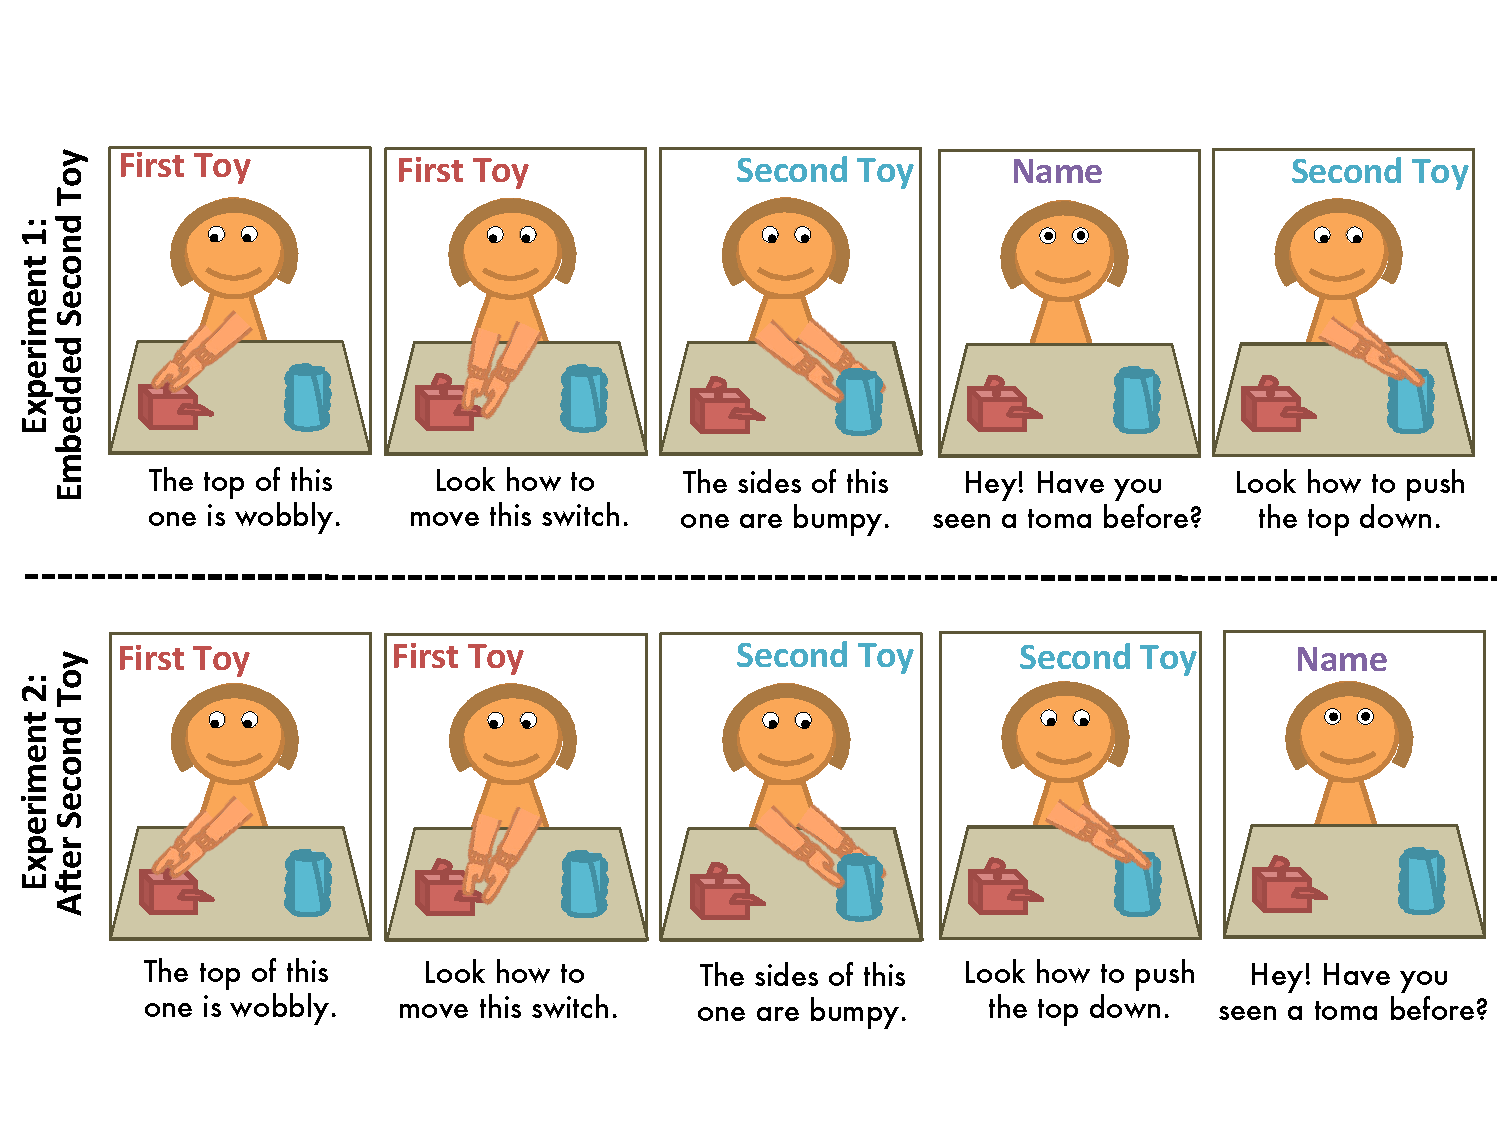
\includegraphics[width=6in]{figures/continuity_demo_slide.pdf} 
    \caption{\label{fig:demo} Schematic order of events for ``Second Toy'' trials across Experiments (``First Toy" trials not pictured). In Experiment 1 (\emph{Embedded} trials), the experimenter made eye contact without other gaze cues and introduced the naming event between two descriptions of a single toy.  In Experiment 2 (\emph{After} trials), events were identical except that the experimenter introduced the naming event after two descriptions of a toy.} 
  \end{center} 
\end{figure}	

\section{Methods}


\subsection{Participants}

A planned sample of 64 children was recruited from the San Jose Children's Discovery Museum.  Participants were uniquely by their birth dates to prevent repeat inclusion in the study.  Children were given a sticker and certificate as compensation their participation.  Parents were asked to fill out a short demographic form about their children's language background, and only children who were reported to hear English at least 75\% of the time were included in the study.  Seven additional children were recruited but excluded for not meeting this criterion: three children due to insufficient English exposure and four children whose language information was not reported.\footnote{As part of our partnership with Children's Discovery Museum, we invite any interested visitors to participate in our studies rather than prescreening children to meet our language requirements \cite{callanan2012}. This standard to recruit inclusively also accounts for variability in gender counts across conditions.}

Children were recruited in four age groups: 2-year-olds (n = 16, 12 girls, mean age 2 years 7 months), 3-year-olds (n = 16, 4 girls, mean age 3 years 6 months), 4-year-olds (n = 16, 6 girls, mean age 4 years 5 months), and 5-year-olds (n = 16, 8 girls, mean age 5 years 4 months).  

We also recruited a comparison group of twelve adults from the museum, none of whom had children who participated in the study. Adults filled out a brief demographic form reporting their own language background, and only adults using English at least 75\% of the time were included in the final sample. Only one additional participant was excluded for reporting less than this amount of English use.  


\subsection{Stimuli}

Four pairs of unusual items (e.g. a faucet aerator and a spaghetti measure) served as the novel toys.  An additional item (an oddly-shaped funnel) was used for training. Pictures of all toys are given in the Appendix.

\subsection{Procedure}

Participants were seated across from the experimenter in a quiet room at the museum.  Children participated in a training trial featuring ostensive labeling of a single toy (``This toy is called a blicket.  Can you point to the blicket?'') to familiarize them to the design and to practice pointing before seeing four discourse disambiguation trials.  Adults participated in the four discourse disambiguation trials without undergoing the initial training. 

For the discourse disambiguation trials, the experimenter placed a unique set of two toys on the table and described each in turn (see Figure \ref{fig:demo}, top).  In these Embedded trials, the experimenter introduced the naming event between two sentences about the same toy.  The labels introduced in the four trials were "toma", "modi", "gazzer", and "zib".  Each participant heard a naming event embedded between descriptions of the first toy for two of the trials (``First Toy'' trials) and between descriptions of the second toy for two of the trials (``Second Toy'' trials).  Label location, trial order, toy pairs, and target side were counterbalanced across participants.  Sample scripts for each trial type are shown in Table \ref{tab:1b}.  

When describing the toys, the experimenter directed her gaze to the toy and demonstrated a feature of the toy.  There was a brief pause between each sentence.  For the naming event, she disengaged from the toy and maintained a neutral position while drawing participants' attention by using their names and establishing eye contact.  The experimenter did not give any gaze cues or other indicators to the referent of the novel name.  Thus, the naming event in itself carried no information to guide disambiguation; the only cue available was its location within discourse.  The toy pair remained in view of the participant throughout the duration of the trial.  At the end of each trial, the experimenter prompted the participant to identify the named item by pointing (e.g. ``Can you point to the toma? Which one it the toma?'').  If children did not respond immediately, they were prompted again to make their best guess. The sessions were videotaped and coded offline. The entire task took about 5 minutes to complete. 


 

\subsection{Results}

Despite the lack of coincident social cues to disambiguate the label, overall children and adults were both more likely to select the toy whose descriptions surrounded the naming event, suggesting that they can recognize and make inferences from discourse continuity.  Figure \ref{fig:res5}, left, illustrates the proportion of children and adults selecting the second toy as the referent of the label across trial types (whether the label was introduced with the First Toy or the Second Toy).  Children and adults were more likely to select the second toy in Second Toy trials and less likely to select the second toy (thus more likely to select the first toy) in First Toy trials, and this pattern was more pronounced in older children. By age 3 -- 4, children's responses appeared to be sensitive to naming condition, and by age 6, children's ability to use topic continuity in this paradigm was comparable to adult performance.


\begin{figure}
  \begin{center} 
    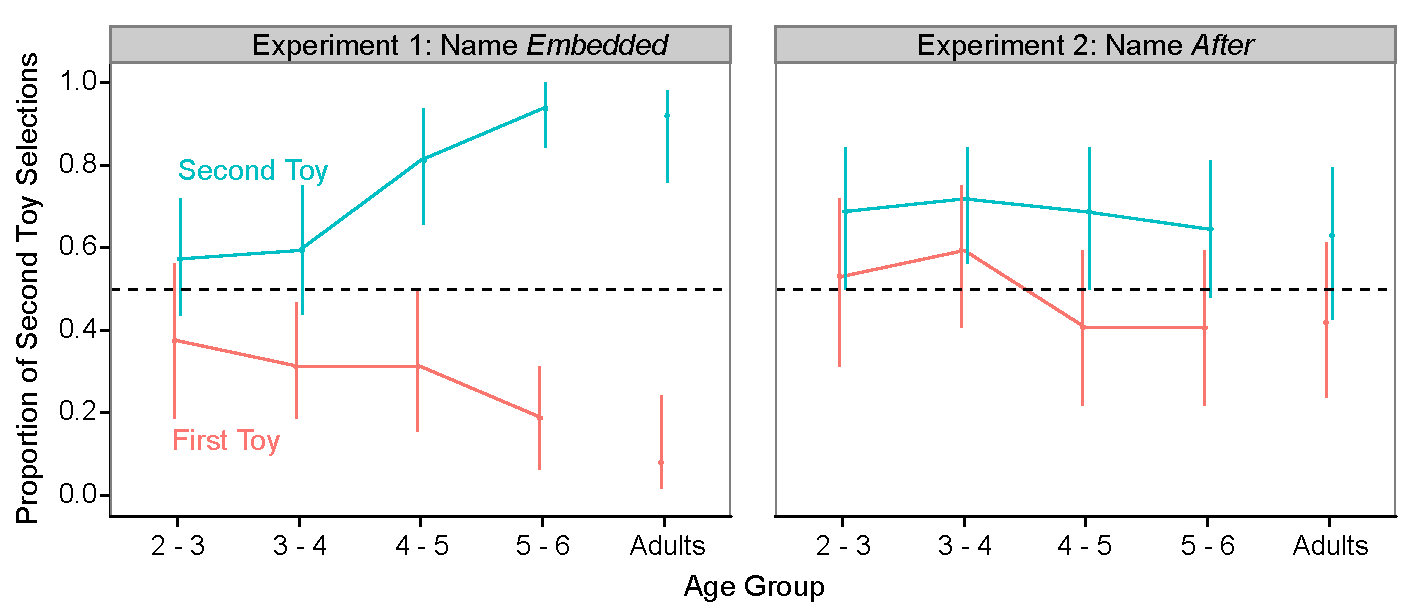
\includegraphics[width=6in]{figures/continuity_kids_and_adults_final.pdf} 
    \caption{\label{fig:res5} Combined data from Experiments 1 and 2.  Mean proportion of selection of the second toy across Experiment (Embedded or After) and trial type (label given with First Toy or Second Toy), plotted by age group (ranges denote age in years). The dashed line indicates chance performance, and error bars show 95\% confidence intervals, computed by a non-parametric bootstrap over participants.} 
  \end{center} 
\end{figure}	



  \begin{table} [t]
   \caption{Coefficient estimates from generalized linear mixed models predicting toy selection as an interaction between trial type and age with random effects of participant and trial type for Experiment 1 (left) and Experiment 2 (right).
   \label{tab:coefficient_estimates} } 
   \begin{center} 
     \begin{tabular}{lrrrr|rrrr} 
          & \multicolumn{4}{c}{Experiment 1: Embedded trials} &  \multicolumn{4}{c}{Experiment 2: After trials}\\
                      \hline 
       \null  & Coef. & Std. Err. & $z$  &  $p(|z|)$ & Coef. & Std. Err. & $z$  &  $p(|z|)$  \\ 
       \hline  
        Age   & -0.27 	&  0.20 & -1.40 & 0.16						               & -0.21 & 0.21 & -0.98 & 0.40\\ 
        Trial type   & -2.24 & 1.17 &  -1.92 & 0.06				                       & 0.00 & 1.13 & 0.00 & 0.99 \\
        Age $\times$ Trial type    & 1.10 & 0.30 & 3.61 &\textbf{ $<$0.001} 		& 0.23 & 0.27 & 0.83 & 0.41\\ 
       \hline 
     \end{tabular} 
  \end{center}
 \end{table}
 

To measure the reliability of these patterns, we fit a generalized linear mixed effects model predicting second toy selection as an interaction between trial type (naming event with the First Toy or Second Toy) and age, with random effects of participant and trial type (the maximal structure appropriate for our experimental design; \citeNP{barr2013}). Age was treated as a continuous variable. This model found no main effect of age and a trend towards a main effect of trial type, indicating that children and adults were overall somewhat more likely to select the second toy in Second Toy trials. The primary effect, however, was a significant interaction between age and trial type, indicating that participants' reference selections by naming location increased with age. Coefficient estimates from these models are shown in Table \ref{tab:coefficient_estimates}, left.

%This model found significant differences in toy selection by both trial type and age group, such by 4-year-olds exhibited marginally stronger performance than 2-year-olds at selecting the toy according to the embedded naming location. Five-year-olds and adults were significantly more likely to show this response pattern. 


   \begin{table} [t]
   \caption{Within each experiment (Embedded trials or After trials), the mean proportion and standard error for participants' selecting the toy matching the naming location across trial types (i.e. choosing the first toy in a First Toy trial and the second toy in a Second Toy trial) and results from paired $t$-tests examining response differences across trial types (naming location with the First Toy or Second Toy). \label{tab:2} } 
   \begin{center} 
     \begin{tabular}{lccrrr|ccrrr} 
          & \multicolumn{5}{c}{Experiment 1: Embedded trials} &  \multicolumn{5}{c}{Experiment 2: After trials}\\
                      \hline 
       \null Age & Prop. & SE & $t$-value & df & $p$-value  & Prop. & SE & $t$-value & df & $p$-value  \\ 
       \hline  
        2--3  & 0.59 & 0.06 & -1.23 & 15 & 0.24 & 0.58 & 0.06 & -1.58 & 15& 0.14\\ 
        3--4  & 0.64 & 0.06 & -2.52 & 15 & \textbf{0.02} & 0.56 & 0.06 & -1.23 & 15 & 0.24 \\ 
        4--5  & 0.75 & 0.05 & -5.48 & 15 & \textbf{$<$0.01} & 0.64 & 0.06 &-1.95 & 15 & 0.07\\
        5--6  & 0.88 & 0.04 & -8.22 & 15 & \textbf{$<$0.01} & 0.64 & 0.06  & -1.58 & 15 & 0.14\\ 
        Adults & 0.92 & 0.06 & -11.72 & 11 & \textbf{$<$0.001} & 0.60 & 0.06 & -1.16 & 11 & 0.27 \\
       \hline 
     \end{tabular} 
  \end{center}
 \end{table}
 
We also ran a series of paired $t$-tests to examine response differences between trial types for each age group (Table \ref{tab:2}, left).  Significant differences in reference selection were found across First Toy and Second Toy Embedded trial types for children ages 3 -- 6 years; unlike the 2-year-olds, older children were more likely to select the first toy in First Toy trials and the second toy in Second Toy trials.

Our results in Experiment 1 suggest that listeners are sensitive to discourse continuity to resolve reference ambiguity.  By varying where a novel label was embedded within a topic, we found that older children and adults systematically selected the toy whose descriptions bracketed the naming event, suggesting that they were sensitive to where in the discourse the name was introduced.  However, it is possible that listeners were using other heuristics to make their selections rather than relying on the discourse structure per se \cite{samuelson1998}.  In order to investigate this possibility, we ran a second experiment to dissociate discourse continuity from simpler associative strategies. 

% DURING
% (Intercept)      0.1500     0.7835   0.191 0.848135    
% age             -0.2737     0.1963  -1.395 0.163161    
% corr.sideB      -2.2434     1.1703  -1.917 0.055241 .  
% age:corr.sideB   1.0995     0.3049   3.606 0.000311 ***

% AFTER
%                  Estimate Std. Error z value Pr(>|z|)
% (Intercept)     0.7366232  0.8800883   0.837    0.403
% age            -0.2097612  0.2135395  -0.982    0.326
% corr.sideB      0.0008899  1.1286078   0.001    0.999
% age:corr.sideB  0.2266775  0.2734905   0.829    0.407

 
 
\section{Experiment 2}

Experiment 1 showed that children and adults chose the toy whose descriptions surrounded the naming events. A high-level explanation for this finding is that listeners assumed that these sentences formed part of a broader discourse about the toy. Nevertheless, the data are also consistent with a lower-level explanation: Participants could be making a temporal association between the label and the toy descriptions, rather than necessarily considering discourse structure. That is, participants could have been selecting the toy that was described nearest to the naming event in time, which in Experiment 1 would always correspond with the toy surrounding the introduction of the label in Embedded trials. 

Experiment 2 was designed to rule out this particular version of a temporal proximity hypothesis.  We made a slight modification to the scripts such that the naming event was moved to be introduced \emph{after} descriptions of either the First Toy or the Second Toy rather than embedded between descriptions of that toy.  
Thus in these \emph{After} trials, the naming event could occur next to descriptions of both toys in ``After First Toy'' trials, or next to only the second toy in ``After Second Toy'' trials. As before, the paradigm is shown in Figure \ref{fig:demo}, and sample scripts are given in Table \ref{tab:1b}.  

This design allows us to make the following predictions: If children recognize discourse continuity as a cue to reference, they should infer that new information contained within a single topic is likely to also refer to that topic. This should lead them to guess at chance in the After trials of Experiment 2. If children rely on temporal association as a heuristic, they should also be at chance in the After First Toy trials, where the label can refer to either one or the other toy.  In the After Second Toy trials, however, they should systematically select the second toy because this is the only item that receives any attention from the speaker proximate to the naming event. 
 
\section{Methods}

\subsection{Participants}

A new planned sample of 64 children was recruited from the San Jose Children's Discovery Museum. As before, children were recruited in four age groups: 2-year-olds (n = 16, 6 girls, mean age 2 years 6 months), 3-year-olds  (n = 16, 6 girls, mean age 3 years 6 months), 4-year-olds (n = 16, 8 girls, mean age 4 years 6 months), and 5-year-olds (n = 16, 10 girls, mean age 5 years 5 months).  Five additional children were excluded due to insufficient English exposure, six children were excluded whose language information was not reported, and four children were excluded for not completing all four trials of the study.  Also as before, we recruited a group of twelve adults, all of whom reported using English at least 75\% of the time and had not seen the study before.  Birth dates and video records confirmed that none of our participants had taken part in Experiment 1. 

\subsection{Stimuli}

Stimuli were identical to Experiment 1. 

\subsection{Procedures}

Procedures were identical to Experiment 1, with one minor change to the script of each trial: The location of the naming event was moved to occur after two descriptions of a toy rather than being embedded between the two descriptions. Thus, participants in Experiment 2 heard all of the same sentences and demonstrations as in Experiment 1, the only difference was the discourse location where the label was introduced; for two trials the label was introduced after descriptions of the first toy (``After First Toy'' trials), and for two trials the label was introduced after descriptions of the second toy (``After Second Toy'' trials).  

\subsection{Results}

As predicted, children and adults were completely at chance in the After First Toy trials, and showed only a weak bias to use temporal proximity to disambiguate reference in After Second Toy trials. Figure \ref{fig:res5}, right, illustrates the proportion of children and adults selecting the second toy as the referent of the label by naming location.  Paired $t$-tests between reference selections across After First Toy and After Second Toy trials for each age group indicated that there were no significant differences in toy selection by trial type for any age group (Table \ref{tab:2}, right), though there was a trend towards such an effect in the 4--5 year-old group. 

% data:  subset(agg.data.s, agg.data.s$agegroup == "2" & condition ==     "After" & corr.side == "B")$side - 0.5
% t = 2.0868, df = 15, p-value = 0.05439

% data:  subset(agg.data.s, agg.data.s$agegroup == "3" & condition ==     "After" & corr.side == "B")$side - 0.5
% t = 2.7815, df = 15, p-value = 0.01397

% data:  subset(agg.data.s, agg.data.s$agegroup == "4" & condition ==     "After" & corr.side == "B")$side - 0.5
% t = 2.0868, df = 15, p-value = 0.05439

% data:  subset(agg.data.s, agg.data.s$agegroup == "5" & condition ==     "After" & corr.side == "B")$side - 0.5
% t = 1.6231, df = 15, p-value = 0.1254

% data:  subset(agg.data.s, agg.data.s$agegroup == "adult" & condition ==     "After" & corr.side == "B")$side - 0.5
% t = 1.3933, df = 11, p-value = 0.1911

Because predictions differed between After First Toy and After Second Toy trials, however, we also tested whether there was any temporal bias specifically in After Second Toy trials. We conducted one-sample t-tests between means from participants in each group and chance. These tests revealed a different developmental pattern from results in the pairwise tests (and from results in Experiment 1). Performance was reliable or close to reliable for 2-, 3-, and 4-year-olds ($t(15) = 2.09$, $2.78$, and $2.09$, $p = .054$, $.01$, and $.054$ respectively). In contrast, performance for 5-year-olds and adults was not reliably different from chance ($t(15) = 1.62$ and $1.39$, $p = .13$ and $.19$, respectively). 

To analyze performance patterns across trial types, we fit a generalized linear mixed effects model as in Experiment 1 by predicting toy selection as an interaction between trial type and age with random effects of participant.  There were no significant effects in the model, indicating that---given the level of power achieved in this study---we could not measure reliable differences in response between After First Toy and After Second Toy trials. Coefficient estimates from the model are shown in Table \ref{tab:coefficient_estimates}, right. Taken together, our findings suggest that younger children might have been somewhat more likely than chance to rely on temporal association, but we cannot draw strong conclusions due to the lack of differences between First Toy and Second Toy trial types. 

% age                             -0.1834     0.1834  -1.000   0.3174  
% corr.sideB                       0.0582     1.0602   0.055   0.9562  
% conditionDuring                 -0.4841     1.1312  -0.428   0.6687  
% corr.sideB:age                   0.1999     0.2569   0.778   0.4364  
% conditionDuring:age             -0.1085     0.2795  -0.388   0.6979  
% conditionDuring:corr.sideB      -2.2733     1.5939  -1.426   0.1538  
% conditionDuring:corr.sideB:age   0.9033     0.4019   2.247   0.0246 *
  \begin{table} [t]
   \caption{Coefficient estimates from a generalized linear mixed models predicting toy selection as an interaction between trial type, age, and experiment.
   \label{tab:coefficient_estimates_full} } 
   \begin{center} 
     \begin{tabular}{lrrrr} 
       \hline 
       \null  & Coef. & Std. Err. & $z$  &  $p(|z|)$ \\
       \hline  
        Age                                                                     & -0.18 &  0.18 & -1.00 & 0.32 \\
        Trial type                                                            & 0.06 &1.06 &  0.06 & 0.96 \\
        Experiment                                                         & -0.48 & 1.13 &  -0.43 & 0.67 \\
        Age $\times$ Trial type                                      & 0.20 & 0.26 & 0.78 & 0.44\\ 
        Age $\times$ Experiment                                   & -0.11 & 0.28 & -0.39 & 0.70\\ 
        Trial type $\times$ Experiment                          & -2.27 & 1.59 & -1.43 & 0.15 \\ 
        Age $\times$ Trial type $\times$ Experiment    & 0.90 & 0.40 & 2.25 & {\bf 0.02} \\ 
       \hline 
     \end{tabular} 
  \end{center}
 \end{table}
 
To test whether participants' performance in Experiment 1 could reliably be distinguished from their performance in Experiment 2, we additionally fit a combined generalized linear mixed effects model across the data from both experiments, adding experiment as an additional between-subjects factor (Table \ref{tab:coefficient_estimates_full}).  The only reliable effect in this model was a three-way interaction between experiment, trial type, and age, indicating that, with increasing age, children were more likely to select the first toy in First Toy trials and the second toy in Second Toy trials, for Experiment 1 more than Experiment 2. This analysis confirms that the behavior and developmental trend we observed in Experiment 1 and attributed to use of discourse information was distinct (at least for older children) than that observed in Experiment 2 and attributed to temporal association.

\section{General Discussion} 

We investigated whether adults and children can use position in discourse as a cue to connect social information with an ambiguous label. In our experiments, adults made effective use of discourse position and children showed increasing sensitivity to discourse position with age. In addition, all age groups except the 2-year-olds successfully used discourse position to infer the referent of a novel label. Taken together, our findings suggest a potential role for discourse continuity in helping children use social information in otherwise ambiguous contexts, and strengthen the argument that models of word learning should incorporate discourse information as a valuable cue to reference and perhaps meaning \cite{luong2013}.

We also investigated an alternative account that children simply rely on temporal proximity to resolve local referential ambiguities.  In particular, our After Second Toy trials in Experiment 2 presented only a single possible referent adjacent to the naming event.  Despite its temporal proximity, children showed only a weak bias to choose the second toy when the naming event followed descriptions of the second toy---and this bias was stronger for younger children, in contrast to the stronger use of discourse information by older children.
%  In fact, our results indicated that participants of all ages selected between the first and second toys at near chance levels for both the After First Toy and After Second Toy trials.  

One possible explanation for older participants' near chance selections in After Second Toy trials is that they inferred that a labeling event coming at the end of two balanced descriptions was equally likely to refer to either object: that the label was related to the higher-order discourse goal of discussing this set of objects as a whole. In principle, another possibility is that they guessed that the label referred to both objects at once, though in practice we did not hear any comments that suggested this in participants' responses, and the toys were sufficiently dissimilar to make this explanation unlikely. In sum, although temporal association might have provided some information, perhaps biasing the response of our youngest participants, such an account does not explain the pattern of data we observed.

Our results from the After trials in Experiment 2 rule out a second possible class of accounts as well: that children's mappings are driven purely by familiarity.  If this were the case, children should map a new label to an item already introduced by the experimenter.  Children's behavior in the Embedded trials is consistent with this account. In Embedded trials, the target toy is described immediately before the experimenter provides a novel label. But in After First Toy trials, a familiarity account would have predicted an even stronger bias towards the first toy, which we also did not observe. These results thus provide additional support for the interpretation of \citeA{akhtar1996} that some sort of discourse understanding, rather than pure familiarity or association, explains children's inferences in word-learning contexts.

The youngest children in our sample did not consistently use discourse position to disambiguate the reference of social cues, unlike the two-year-olds in \citeA{akhtar1996}. Nevertheless, our findings do not provide evidence against two-year-olds' ability to use discourse information to learn words more generally. Our paradigm was relatively complex and fast moving, involving attending closely to an experimenter across five distinct utterances in each of four trials, each with a new pair of objects. The attentional demands of the paradigm may therefore have limited performance for the youngest children we tested. Eye-movement based measurements, combined with even stronger discourse contexts \cite<e.g.>{song2005}, might provide a method for measuring two-year-olds' performance in future work.

Because of the complexity of the factors involved in establishing reference in discourse context, computational models in principle might play a valuable role in helping to formalize the role of repeated references in children's reference determination and word learning. But despite the evidence on children's discourse sensitivity, most models of word learning treat utterances as independent from one another in time, completely discarding any discourse information. For example, in the models of \citeA{siskind1996}, \citeA{yu2007}, and \citeA{fazly2010}, no mention is made of the connections between sentences as a possible source of information. Even a model that was intended to capture the intentional nature of early word learning did not incorporate any assumption that communicative intentions would be related to one another across time \cite{frank2009}. 
% One early model did build in some temporal dependency between utterances via a memory-based filter \cite{roy2002}, but again it is an open question whether such memory biases could lead to discourse-related inferences (our current study provides some new evidence on this issue).

One recent model provides some hints, however. Building on \citeA{frank2009}, \citeA{luong2013} created a word learning model in which the speaker's intended referent is continuous from sentence to sentence. This model incorporated social cues with discourse information and showed some modest improvements in word learning and reference resolution on the basis of including this information. Although this model provides some initial insights, it does not fully explore the potential of discourse information in more sophisticated referential situations. Further computational work is needed to understand when it is that discourse information is most helpful for learners. 

Discourse continuity may provide the glue that holds together noisy social cues into a coherent referential structure, allowing children to aggregate information about what words mean across multiple utterances.  Our work begins to address this idea by demonstrating that children are sensitive to discourse structure in simple referential contexts, and future work can build on these initial findings to examine the extent to which listeners incorporate cues to discourse continuity in their comprehension processing.  The ability to make inferences about how sentences fit together could be a valuable learning mechanism. From learning that a chinchilla is a furry animal to picking up the subtle judgments that people express in the nuances of the way they fit their sentences together, children's ability to reason about meaning in discourse context may help them to use language to learn about the world around them. 

\bibliographystyle{apacite2}
\bibliography{disc_wl}

\newpage
\theappendix 

\section{Appendix A: Materials}


\begin{figure}
  \begin{center} 
    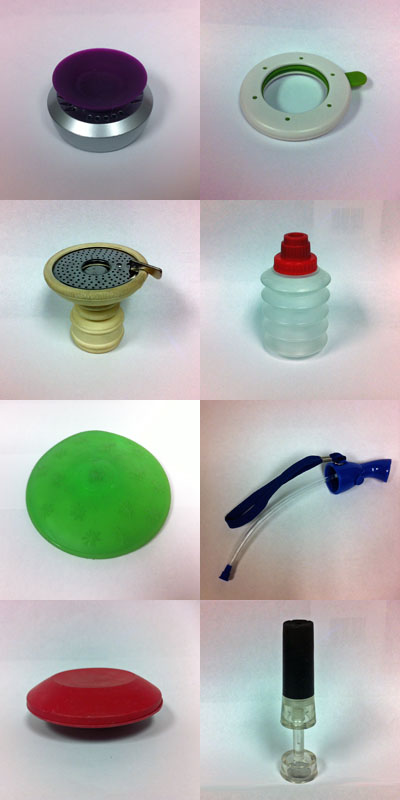
\includegraphics[width=2.5in]{figures/discourse_toys_images.jpg} 
    \caption{\label{fig:toys} The four pairs of toys used in Experiments 1 and 2. Each toy had a unique affordance. For example, the lid in the upper left hand corner could be popped open and closed or spaghetti sizer in the upper right photo could be irised open and shut.} 
  \end{center} 
\end{figure}

 \begin{table}
   \caption{Sample scripts for Experiments 1 and 2 across trial type (First Toy or Second Toy).  Naming location was counterbalanced across participants.  Red sentences are descriptions of the First Toy; blue sentences are descriptions of the Second Toy. Both were accompanied by unambiguous social cues. \label{tab:1b} } 
   \begin{center} 
   \small\addtolength{\tabcolsep}{-5pt}
     \begin{tabular}{ll} 
\scalebox{0.1}
       \null   \textbf {Experiment 1}  \\ 
       \hline 
       \textbf{Embedded First Toy} & \textbf{Embedded Second Toy} \\ 
       \hline {\color{Red}The top of this one is wobbly.} &  {\color{Red} The top of this one is wobbly.} \\ 
      \textbf{Have you seen a toma before?} &  {\color{Red} Look how to move this switch. }\\ 
       {\color{Red}  Look how to move this switch.} & {\color{BlueGreen}The sides of this one are bumpy.}\\
	  {\color{BlueGreen}The sides of this one are bumpy.} &   \textbf{Have you seen a toma before?} \\
       {\color{BlueGreen}Look how to push the top down.} & {\color{BlueGreen} Look how to push the top down.} \bigskip \smallskip\\ 
        \null    \textbf {Experiment 2}  \\         
       \hline 
        \textbf{After First Toy} & \textbf{After Second Toy} \\ 
       \hline {\color{Red}  The top of this one is wobbly.} & {\color{Red}The top of this one is wobbly.}\\ 
      {\color{Red}Look how to move this switch.} & {\color{Red}Look how to move this switch. }\\ 
  \textbf{Have you seen a toma before?} & {\color{BlueGreen} The sides of this one are bumpy.}\\
       {\color{BlueGreen}The sides of this one are bumpy.}  & {\color{BlueGreen}  Look how to push the top down.}\\ 
      {\color{BlueGreen}Look how to push the top down.} &   \textbf{Have you seen a toma before?} \\
       \hline  \end{tabular} 
   \end{center}
 \end{table}


\end{document}
